\chapter{Zusammenfassung und Ausblick}

\begin{itemize}
  \item 2-3 Seiten Zusammenfassung der Arbeit und Ausblick auf weitere
Projekte f�r die Zununft
  \item Vgl. Erwartete Ergebnisse - Abweichungen  
  \item marketingtechnische konzepte: kann das ergebnis im hinblick darauf
  kontrolliert werden? kundenzufriedenheit \& co.? wie k�nnte eine m�gliche
  evaluation erfolgen?
\end{itemize}

Die Erwartungshaltung f�r diese Diplomarbeit bestand darin in einer vorgegebenen
Zeit zu evaluieren, ob der Einsatz von Smartphoneapps in der Kommunikation mit
Maschinen lohnend ist oder nicht. Ausgehend vom Wissensstand zu Beginn dieser
Arbeit wurde vermutet, dass die Umsetzung einer App durchaus m�glich, wenn
auch nicht einfach ist. Die gr��te Schwierigkeit im Vorfeld lag vor allem daran,
die Darstellung der verschiedenen Funktionen f�r das Endger�t so zu optimieren,
dass die Lesbarkeit der Information jederzeit gew�hrleistet sein sollte. Bei
einer begrenzten Displaygr��e vor allem bei Smartphones m�ssen Informationen
klar und deutlich zu gewinnen sein. 

% \clearpage
% \thispagestyle{empty}
% \begin{figure}[hp]
% 
\includegraphics[width=\textwidth]{beispiel}
% \end{figure} 
% \clearpage
% 
% \chapter{Beispielanhang 2}
% Dies ist das Deckblatt. Es sollte die kurze Beschreibung der n�chsten Seite enthalten. Der Titel ist meist ausreichend.
% 
% % so gehts auch
% \clearpage
% \thispagestyle{empty}
% \begin{figure}[hp]
% 
\includegraphics[height=\textwidth,angle=90]{beispiel}	% jetzt querformat
% \end{figure} 
% \clearpage
% 
% \addtocontents{toc}{\vspace{-1ex}}
% \chapter{Beispielanhang 3}
% Dies ist das Deckblatt. Es sollte die kurze Beschreibung der n�chsten Seite enthalten. Der Titel ist meist ausreichend.
% 
% 
% % Wenn der Anhang als PDF vorliegt kann man ihn einfach so einf�gen: (Paket pdfpages n�tig)
% \ifpdf % funktioniert leider nur mit pdfLaTeX 
% 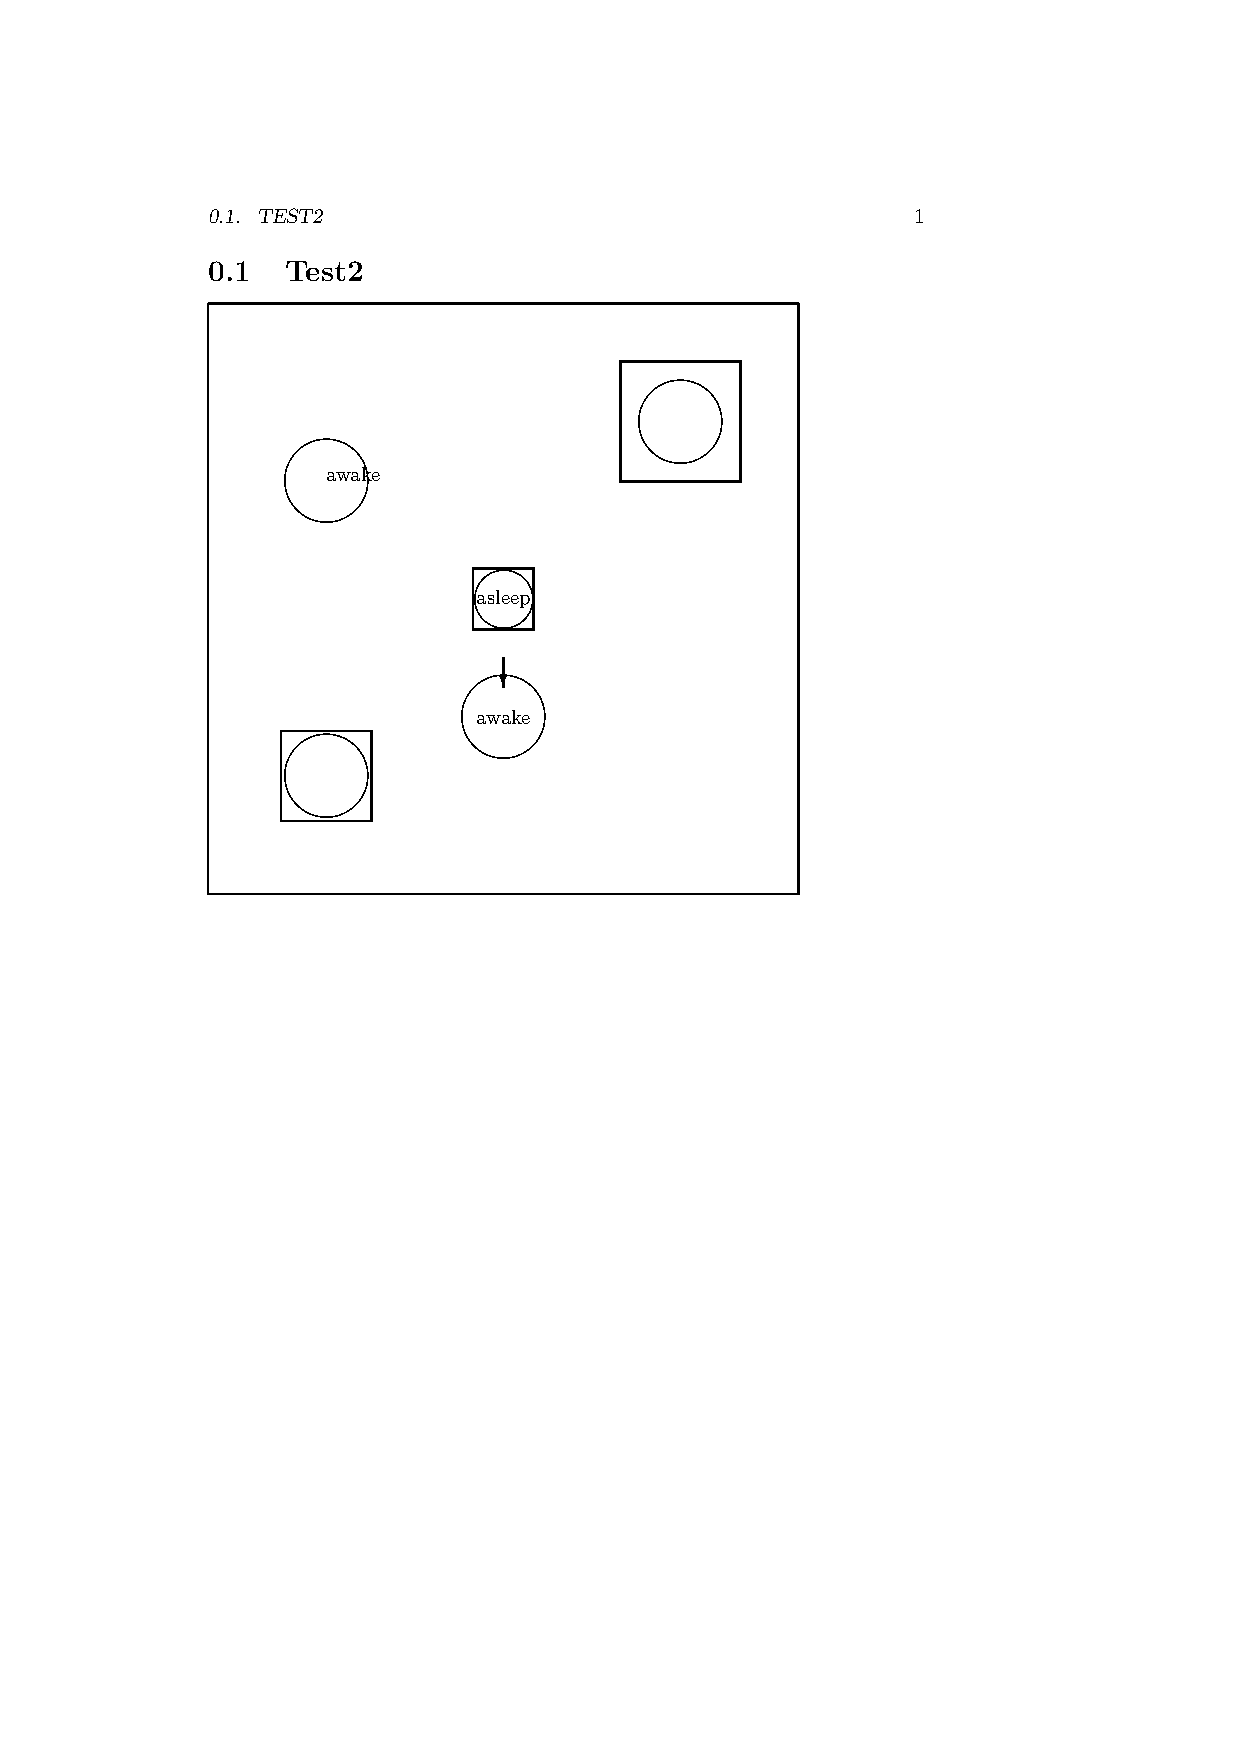
\includepdf[pages=-]{anhang/beispielanhang}	% pages=- bedeutet: alle Seiten | Wie bei Bilder die Dateierweiterung (.pdf) am besten weglassen
% % Weites Beispiel: Nur Seiten 1-2 und 4, Papier querformat mit 2 Seiten pro Seite
% %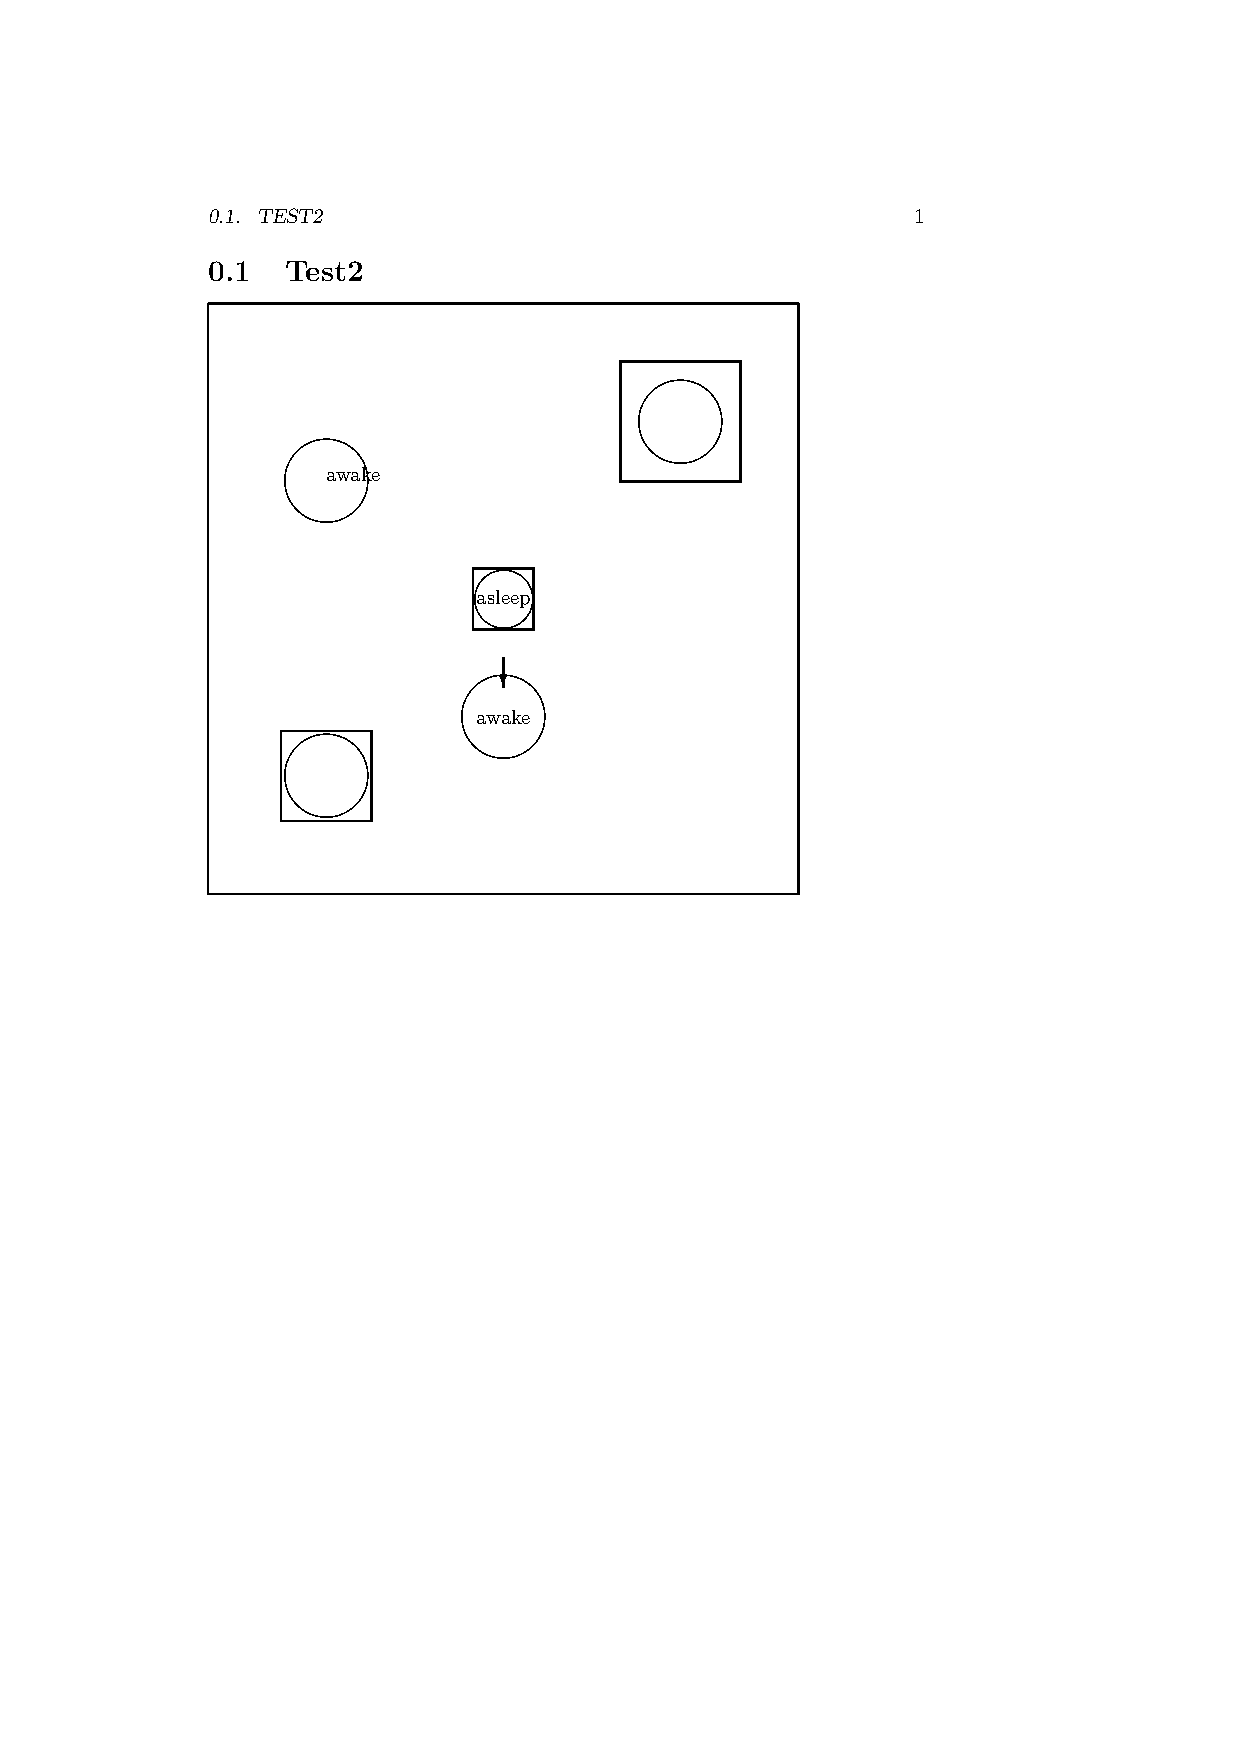
\includepdf[pages={1-2,4},landscape,nup=1x2]{anhang/beispielanhang}
% 
% \else  % bei der Verwendung vom normalen LaTeX:
% \newpage
% \addtocounter{page}{5}	% Seitenz�hler hochz�hlen und Anhang nach dem Drucken manuell hinzuf�gen
% % Hier wurde angenommen, dass der Anhang f�nf Seiten lang ist
% \fi
% 
% \chapter{Weiterer Anhang}
